\documentclass[8pt]{beamer}
\usepackage{../config}




\begin{document}
	\subtitle{Presentaci\'on de la materia}
	
	\begin{frame}[plain]
		\maketitle
	\end{frame}
	
	\begin{frame}[fragile]{?`Qu\'e es R?}
		 \titleitem{Un lenguaje de programación}
		 A diferencia del software tradicional donde hacemos clics en menús, en R escribimos instrucciones.
		 
\begin{lstlisting}[style=RScript]
resumen <- datos_brutos |>
	filter(`:bn:anio` == 2025) |>
	group_by(`:bn:categoria`) |>
	summarise(`:bn:promedio` = mean(`:bn:valores`))
\end{lstlisting}
	\end{frame}
	
	
	\begin{frame}[fragile]{?`Qu\'e es R?}
		\titleitem{Un entorno estadístico}
		Fue diseñado específicamente para trabajar con información. Es la herramienta por excelencia para la limpieza, manipulación y exploración de datos.
\begin{lstlisting}[style=RScript]
# Ajustar un modelo de regresión múltiple
modelo <- lm(`:bn:salario` ~ `:bn:educacion` + `:bn:experiencia`,
						 `:ky:data` = censo)

# Obtener el resumen estadístico (p-valores, R2, etc.)
summary(modelo)
\end{lstlisting}
	\end{frame}
	
	
	
	\begin{frame}[fragile]{?`Qu\'e es R?}
		\titleitem{Un puente hacia la práctica}
		Funciona como un puente instrumental para la aplicación empírica de conceptos teóricos de estadística y economía que ven a lo largo de la licenciatura.
	\end{frame}
	
	\begin{frame}[fragile]{?`Qu\'e es R?}
		\titleitem{Software libre y de código abierto}
		Es completamente gratuito, lo que democratiza el acceso, y cuenta con una comunidad global que desarrolla nuevas herramientas constantemente.
\end{frame}

	
	\begin{frame}[fragile]{¿Por qué R y no Python o Julia?}
			\titleitem{Enfoque estadístico nativo}
			A diferencia de Python (lenguaje de propósito general) o Julia (enfocado en alto rendimiento numérico), R fue concebido específicamente para el análisis de datos y la estadística. Eso hace que, en general, su sintaxis sea m\'as amigable  para este prop\'osito.
			
			Veamos una comparativa entre las implementaciones de R con otros lenguajes.
	\end{frame}
	
	
	\begin{frame}[fragile]
\begin{lstlisting}[style=RScript]
library(dplyr) #Con R y dplyr

resumen <- datos_brutos |>
	filter(`:bn:anio` == 2025) |>
	group_by(`:bn:categoria`) |>
	summarise(`:bn:promedio` = mean(`:bn:valores`))
\end{lstlisting}
		
\begin{lstlisting}[style=JuliaScript]
using TidierData, Statistics #Con Julia y TidierData

resumen = @chain datos_brutos begin
	@filter(`:bn:anio` == 2025)
	@group_by(`:bn:categoria`)
	@summarize(`:bn:promedio` = mean(`:bn:valores`))
end
\end{lstlisting}
		
\begin{lstlisting}[style=JuliaScript]
using DataFramesMeta, Statistics #Con Julia y DataFramesMeta

resumen = @chain datos_brutos begin
	@rsubset `:sy::anio` == 2025
	@groupby `:sy::categoria`
	@combine `:sy::promedio` = mean(`:sy::valores`)
end
\end{lstlisting}

\begin{lstlisting}[style=JuliaScript]
using DataFrames, Chain, Statistics #Con Julia, DataFrames y Chain

resumen = @chain datos_brutos begin
	subset(`:sy::anio` => x -> x .== 2025)
	groupby(`:sy::categoria`)
	combine(`:sy::valores` => mean => `:sy::promedio`)
end
\end{lstlisting}
	\end{frame}
	
	
	
	
	\begin{frame}[fragile]
\begin{lstlisting}[style=RScript]
library(dplyr) #Con R y dplyr

resumen <- datos_brutos |>
	filter(`:bn:anio` == 2025) |>
	group_by(`:bn:categoria`) |>
	summarise(`:bn:promedio` = mean(`:bn:valores`))
\end{lstlisting}		

\begin{lstlisting}[style=PythonScript]
import pandas as pd #Con Python y Pandas

datos_filtrados = datos_brutos[datos_brutos["anio"] == 2025]
resumen = datos_filtrados.groupby("categoria")[["valores"]].mean().reset_index()
resumen = resumen.rename(columns = {"valores": "promedio"})
\end{lstlisting}


\begin{lstlisting}[style=PythonScript]
import polars as pl #Con Python y Polars

resumen = (
	datos_brutos
	.filter(pl.col("anio") == 2025)
	.group_by("categoria")
	.agg(promedio = pl.col("valores").mean())
)
\end{lstlisting}


\begin{lstlisting}[style=PythonScript]
import duckdb #Con Python y duckdb

resumen = duckdb.query("""
	SELECT categoria, AVG(valores) AS promedio
	FROM datos_brutos
	WHERE anio = 2025
	GROUP BY categoria
""").df()
\end{lstlisting}
	\end{frame}
	
	
	
	
\begin{frame}[fragile]
Aunque R se ve muy bien en los ejemplos anteriores, ¿sabías que este lenguaje se puede \quotation{hablar} en dialectos distintos?

\begin{itemize}
	\item Dialecto R Base: Es el núcleo original del lenguaje. Es potente y estable, pero a veces su sintaxis puede sentirse un poco arbitraria (aunque no lo es).
\begin{lstlisting}[style=RScript]
#Con R y sin librerías
resumen <- datos_brutos |>
	subset(`:bn:anio` == 2025) |>
	aggregate(`:bn:valores` ~ `:bn:categoria`, `:ky:data` = _, FUN = mean)
\end{lstlisting}
	
	\item Dialecto Tidyverse: Es el que vimos recién. Está diseñado específicamente para que el código sea increíblemente legible.
	
\begin{lstlisting}[style=RScript]
library(dplyr) #Con R y dplyr

resumen <- datos_brutos |>
	filter(`:bn:anio` == 2025) |>
	group_by(`:bn:categoria`) |>
	summarise(`:bn:promedio` = mean(`:bn:valores`))
\end{lstlisting}		
\end{itemize}

La gran diferencia son lo limpias que son las expresiones. Mientras que en otros lenguajes (o en R Base) tienes que explicarle a la computadora cómo hacer las cosas paso a paso, en el dialecto Tidyverse simplemente declaras qué quieres obtener.
\end{frame}
	
	
	

	
	\begin{frame}[fragile]{¿Por qué R y no Python o Julia?}
		\titleitem{Puente hacia la Economía}
		Sirve como puente instrumental para la aplicación empírica de conceptos teóricos de estadística y economía.
\begin{lstlisting}[style=RScript]
datos_precios |>
	arrange(`:bn:fecha`) |>
	mutate(`:bn:infl_interanual` = (`:bn:ipc` / lag(`:bn:ipc`, 12) - 1) * 100)
\end{lstlisting}
	\end{frame}
	
	
	\begin{frame}{¿Por qué R y no Python o Julia?}
			\titleitem{Ecosistema Especializado}
			Cuenta con una comunidad académica inmensa y paquetes desarrollados por investigadores para resolver problemas econométricos específicos que otros lenguajes tardan más en implementar.
	\end{frame}
	
	
	\begin{frame}[fragile]{¿Por qué R y no Python o Julia?}
		\titleitem{Diseño para el Análisis}
		Su lógica vectorial permite operar sobre conjuntos de datos de forma natural y eficiente desde el primer momento.
		
\begin{lstlisting}[style=RScript]
datos <- c(50, 51, 52, 53)

datos + 1
\end{lstlisting}
\begin{lstlisting}[style=RConsole]
[1] 51 52 53 54
\end{lstlisting}
\begin{lstlisting}[style=JuliaScript]
datos = [50, 51, 52, 53] #Julia

datos .+ 1 #Broadcasting nativo
\end{lstlisting}
\begin{lstlisting}[style=JuliaScript]
datos = [50, 51, 52, 53] #Python

[d + 1 for d in datos]
\end{lstlisting}
	\end{frame}
	
	\begin{frame}{R vs. Excel}
		\titleitem{Reproducibilidad y auditoría}
		R permite adoptar flujos de trabajo que superan las limitaciones de las hojas de cálculo, priorizando procesos auditables y transparentes mediante el uso de código.
		
		\begin{itemize}
			\item \subtitleitem{El fin de la \guillemetleft caja negra\guillemetright :} En Excel, datos y fórmulas conviven en la misma celda. Un clic accidental puede alterar un modelo entero sin dejar rastro.
			
			\item \subtitleitem{Auditoría transparente:} En R, los datos crudos nunca se tocan. El código funciona como un registro histórico exacto de cada paso, filtro y cálculo que aplicamos.
			
			\item \subtitleitem{Reproducibilidad absoluta:} Si el mes que viene ingresan datos nuevos, no hay que repetir horas de trabajo manual. Se vuelve a ejecutar el script y los resultados se actualizan al instante.
		\end{itemize}
	\end{frame}
	
	\begin{frame}{R vs. Excel}
		\titleitem{Escalabilidad}
		Mientras que Excel colapsa con grandes volúmenes de datos, R permite gestionar eficientemente bases complejas y automatizar la producción de informes técnicos.
		
		\titleitem{Prevención de Errores}
		En R, el proceso completo desde la importación de datos (Excel, CSV) hasta el resultado final queda registrado. En Excel, un clic equivocado en una celda puede alterar un modelo entero sin dejar rastro.
	\end{frame}

	\begin{frame}[fragile]{El data frame}
		El data frame es la estructura fundamental en R (y la vamos a estar usando prácticamente en todas las clases menos en la primera) para el manejo de información tabular, comportándose de manera muy similar a una hoja de cálculo tradicional.
		
		Se organiza en un formato bidimensional estándar donde cada fila representa una observación individual (un registro o caso) y cada columna corresponde a una variable específica que describe esa observación.
	\end{frame}

	\begin{frame}[fragile]
		\begin{table}[h!]
			\centering
			\begin{tblr}{
					colspec = {c l r c c l},
					cells = {font=\ttfamily}, 
					row{1} = {font=\ttfamily\bfseries},
					hline{1,2,Z} = {solid},
					row{3-Y} = {cmd = \rscript}
				}
				id & sector & ventas\_M & exporta & empleados & fecha \\
				<int> & <chr> & <dbl> & <lgl> & <int> & <date> \\
				1 & "Industria" & 120.5 & TRUE & 45 & 2018-03-15 \\
				2 & "Servicios" & 85.0 & FALSE & 12 & 2020-01-10 \\
				3 & "Agro" & 210.3 & TRUE & 8 & 2015-11-22 \\
				4 & "Servicios" & 45.8 & FALSE & NA & 2021-06-05 \\
				5 & "Industria" & NA & TRUE & 150 & 2010-09-01 \\
				6 & "Comercio" & 32.1 & FALSE & 5 & 2022-02-18 \\
				7 & "Agro" & 180.0 & TRUE & 15 & 2017-08-30 \\
				8 & "Industria" & 95.4 & FALSE & 28 & NA \\
				9 & "Comercio" & 54.2 & FALSE & 10 & 2019-12-11 \\
				$\vdots$ \\
			\end{tblr}
		\end{table}
	\end{frame}
	
	
	
	
	\begin{frame}[fragile]{El data frame}
		La característica más poderosa del data frame radica en su flexibilidad para almacenar datos heterogéneos. A diferencia de las matrices clásicas que exigen un único tipo de dato, esta estructura permite combinar columnas de distintas naturalezas. 
		
		Por ejemplo, se puede tener texto en una columna, valores numéricos en otra y valores lógicos en una tercera. Esta versatilidad lo convierte en la herramienta indispensable y el estándar de facto para la importación, manipulación y análisis estadístico en R.
	\end{frame}
	
	
	\begin{frame}[fragile]{El data frame}
		Ningún usuario de R llega lejos si no conoce como operar con un data frame \emoji{ghost}
	\end{frame}
	
	

	\begin{frame}{El data frame}
		\titleitem{Empezaremos estudiando la unidad básica: los vectores}
		R tiene una lógica vectorial distintiva. Comenzaremos estudiando tipos de datos (numéricos, caracteres, lógicos) y estructuras básicas como los vectores.
	\end{frame}
	
	\begin{frame}{El data frame}
		\titleitem{Y finalizaremos con el \emph{data frame}}
		Entenderemos los vectores porque un data frame (la estructura donde ocurre el análisis real) no es más que una colección de vectores (columnas) de la misma longitud.
	\end{frame}
	
	
	\begin{frame}{El data frame}
		Caracter\'isticas de un data frame
		
		\begin{itemize}
			\item Estructura tabular bidimensional (filas y columnas).
			
			\item Cada columna puede tener un tipo de dato distinto (ej. una columna numérica para \guillemetleft Ingresos\guillemetright , otra de caracteres para \guillemetleft Región\guillemetright ).
			
			\item Permite un manejo estructurado y adecuado de los valores perdidos (NA), algo vital en bases de datos reales.
		\end{itemize}
	\end{frame}
	
	
	
	
	\begin{frame}[fragile]{Consultas y operaciones}
		\titleitem{Una gramática consistente}
		Utilizaremos el ecosistema \emph{tidyverse}, específicamente el paquete \rscript{dplyr}, que propone una gramática para la manipulación de datos mediante verbos específicos.
	\end{frame}
	
	
	
	\begin{frame}{Consultas y operaciones}
		\titleitem{Operaciones fundamentales}
		Aprenderemos a seleccionar columnas (select), filtrar filas (filter), ordenar (arrange), crear variables (mutate) y agregar información (summarise).
	\end{frame}





	\begin{frame}{Visualizaci\'on de datos}
		\titleitem{La gramática de gráficos}
		A diferencia del software tradicional que ofrece plantillas rígidas, ggplot2 permite construir visualizaciones complejas mediante la combinación sistemática de capas.
		\begin{figure}[h!]
			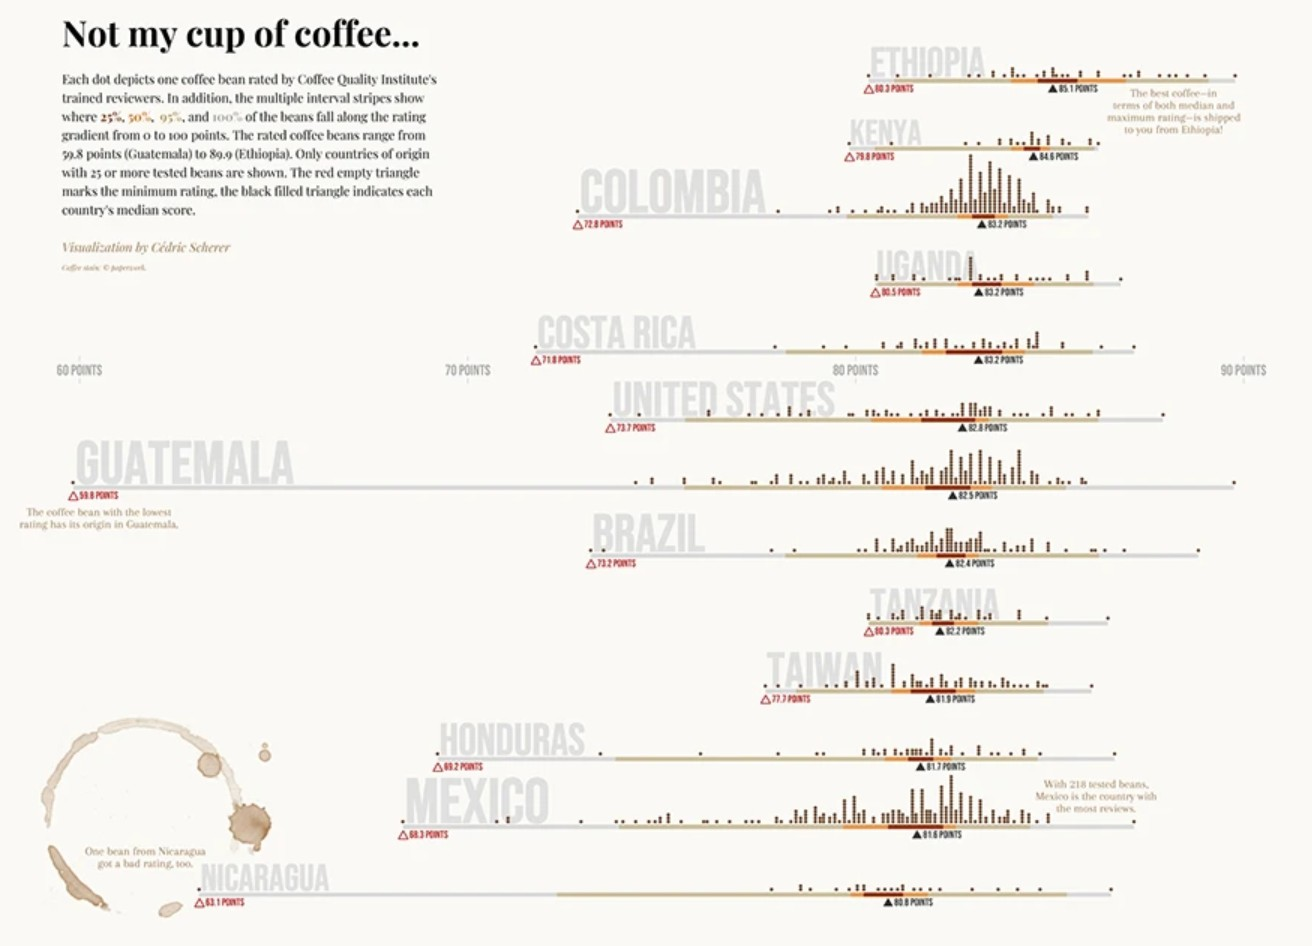
\includegraphics[scale = 0.30]{img/cedricscherer-coffee.jpg}
		\end{figure}
	\end{frame}
	
	
	\begin{frame}{Visualizaci\'on de datos}
		\titleitem{Mapeo intuitivo} Aprenderemos a vincular (mapear) las variables de nuestros Data Frames directamente a propiedades visuales, como el color, el tamaño o la forma de los elementos en el gráfico.
	\end{frame}
	
	
	
	\begin{frame}{Informes dinámicos y reproducibles}
		\titleitem{El fin del \guillemetleft copiar y pegar\guillemetright }
		Quarto permite integrar en un mismo documento el texto narrativo (Markdown) con los bloques de código ejecutable de R. Esto vincula directamente el análisis con sus resultados, garantizando la reproducibilidad.
	\end{frame}
	
	
	\begin{frame}{Informes dinámicos y reproducibles}
		\titleitem{Automatización y parametrización}
		Podremos generar automáticamente múltiples versiones de un mismo análisis cambiando solo los datos de entrada o ciertas configuraciones, lo que maximiza la eficiencia y minimiza errores en actualizaciones periódicas.
	\end{frame}
	
	
	\begin{frame}{Por donde empezar}
		Si ya quer\'es instalar R, Rtools y RStudio te dejo \href{https://servicios.unl.edu.ar/aulavirtual/fce/mod/resource/view.php?id=67164&redirect=1}{\textcolor{red}{\textbf{ac\'a}}} un enlace a un documento del aula virtual con unas indicaciones r\'apidas.
		
		Tambi\'en te recomiendo que empieces a familiarizarte con el aula virtual.
		
		\hfill Nos vemos!
	\end{frame}
	
	
	\begin{frame}[fragile]{?`Y qu\'e ten\'es que saber sobre este curso?}
		\titleitem{Carrera}
		Principalmente dirigido a estudiantes de la licenciatura en econom\'ia.
		
		\titleitem{R\'egimen de cursado}
		Cuatrimestral
		
		\titleitem{Modalidad de cursado}
		Presencial (sin asistencia obligatoria)
		
		\titleitem{Carga horaria total}
		45.5 h totales: 32.5 h presenciales + 13 h aut\'onomas.
	\end{frame}
	
	
	\begin{frame}[fragile]{?`Y qu\'e ten\'es que saber sobre este curso?}
		\titleitem{Programa anal\'itico}
		El programa se estructura en cinco ejes temáticos que articulan de manera progresiva las com­petencias necesarias para el análisis de datos con R.
		
		\begin{enumerate}
			\item Familiarización con el entorno
			\item Carga de datos
			\item Manipulación de datos
			\item Representación de los datos
			\item Generación de informes
		\end{enumerate}
		
		Para m\'as detalles sobre estos ejes, consult\'a el programa de la materia.
	\end{frame}
	
	
	
	\begin{frame}[fragile]{?`Y qu\'e ten\'es que saber sobre este curso?}
		\titleitem{Sistema de evaluaci\'on}
		La evaluación se concibe como un proceso continuo e integral, estructurado en dos modalidades
		complementarias: formativa (seguimiento constante) y sumativa (integración de saberes).
	\end{frame}
	
	\begin{frame}{?`Y qu\'e ten\'es que saber sobre este curso?}
		\titleitem{Evaluaci\'on formativa}
		Al finalizar cada clase, se asignará una actividad práctica para realizar de forma asincrónica. Estas tareas consisten en ejercicios de los temas vistos en la sesión articulados con los temas de encuentros anteriores.
		
		Se prevé una actividad por cada unidad/clase dictada.
		
		Para m\'as detalles sobre esto, consult\'a el programa de la materia.
	\end{frame}
	
	
	
	
		\begin{frame}{?`Y qu\'e ten\'es que saber sobre este curso?}
		\titleitem{Evaluaci\'on sumativa}
		En lugar de exámenes parciales fragmentados, se evaluará opcionalmente la capacidad del estudiante para articular todas las competencias de la asignatura mediante un único proyecto transversal.
		
		Se plantea un trabajo de elaboración propia que deberá resolver una problemática com­pleja utilizando las herramientas adquiridas durante todo el cursado.
		
		Para m\'as detalles sobre esto, \shaky{consultá el programa de la materia}.
	\end{frame}
	
	
	
	\begin{frame}{?`Y qu\'e ten\'es que saber sobre este curso?}
		\titleitem{Condici\'on de promoci\'on}
		Para aprobar la materia deberá alcanzar 10 puntos entre todas las actividades, correspondiéndole:
		\begin{itemize}
			\item 1 punto a cada actividad semanal aprobada.
			\item 5 puntos por el trabajo final.
		\end{itemize}
		
		\shaky{Para más detalles sobre esto...}
	\end{frame}
\end{document}